\documentclass[12pt]{article}

\title{Assignment 2: CS 663, Fall 2021}
\author{\textbf{Question 2}}
\date{}
\usepackage{amsmath}
\usepackage{amssymb}
\usepackage{hyperref}
\usepackage{ulem}
\usepackage{enumitem}
\usepackage{float}
\usepackage{graphicx}
\usepackage{subcaption}
\usepackage{bm}
\usepackage[margin=0.5in]{geometry}
\begin{document}
\maketitle

\begin{itemize}
    \item Implement local histogram equalization of sizes $7 \times 7, 31 \times 31, 51 \times 51, 71 \times 71$ on the images `LC1.jpg' and `LC2.jpg' from the homework folder. Comment on your results in your report and compare it to global histogram equalization, which you can use from the image processing toolbox of MATLAB. Point out regions where the local method produces better local contrast than the global histogram equalization. \textsf{[15 points]}
    \vspace*{0.5cm}\\
    \textbf{Answer:} \\[20pt]
    LC1:\\[10pt]
    \begin{figure}[H]
        \centering
        \begin{minipage}{.45\textwidth}
          \centering
          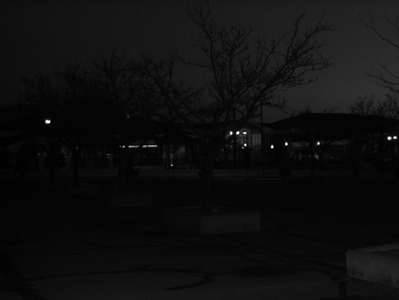
\includegraphics[width=\linewidth]{9/images/LC1.png}
          \caption*{Original LC1 image}
        \end{minipage}
    \end{figure}
    \newpage
    %--------------------------------------------------------
        
    \begin{figure}[H]
        \centering
        \begin{minipage}{.45\textwidth}
          \centering
          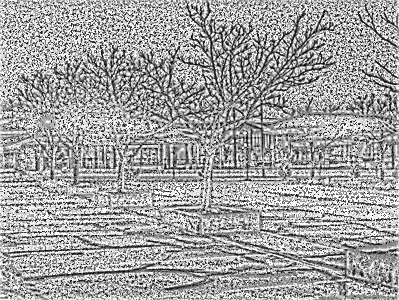
\includegraphics[width=\linewidth]{9/images/LC1_7.png}
          \caption*{Local histogram equalisation with $7\times 7$ bin}
          \label{fig:totalpowervst}
        \end{minipage}
        \begin{minipage}{.45\textwidth}
          \centering
          \includegraphics[width=\linewidth]{9/images/LC1_global_7.png}
          \caption*{Global histogram equalisation}
          \label{fig:totalpower2}
        \end{minipage}
        %\caption{}
        \label{fig:totalPower}
    \end{figure}
    
    Though the $7\times 7$ locally equalised image looks absolutely bad compared to global image, it does have some edge/corner related information. The count of the small branches can be estimated from the local image.\\
    %---------------------------------------------------------
    
    \begin{figure}[H]
        \centering
        \begin{minipage}{.45\textwidth}
          \centering
          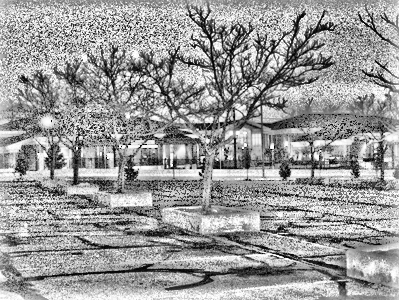
\includegraphics[width=\linewidth]{9/images/LC1_31.png}
          \caption*{Local histogram equalisation with $31\times 31$ bin}
          \label{fig:totalpowervst}
        \end{minipage}
        \begin{minipage}{.45\textwidth}
          \centering
          \includegraphics[width=\linewidth]{9/images/LC1_global_31.png}
          \caption*{Global histogram equalisation}
          \label{fig:totalpower2}
        \end{minipage}
        %\caption{}
        \label{fig:totalPower}
    \end{figure}
    $31\times 31$ locally equalised image is more recognisable than $7\times 7$ but still not better than global in an overall sense. The first tile in the bottom has some slope which can be identified by the contrasting white line in the local image.
    %-----------------------------------------------------------
    
    \begin{figure}[H]
        \centering
        \begin{minipage}{.45\textwidth}
          \centering
          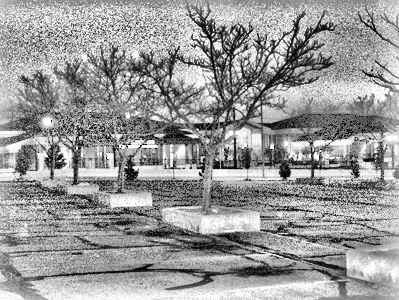
\includegraphics[width=\linewidth]{9/images/LC1_51.png}
          \caption*{Local histogram equalisation with $51\times 51$ bin}
          \label{fig:totalpowervst}
        \end{minipage}
        \begin{minipage}{.45\textwidth}
          \centering
          \includegraphics[width=\linewidth]{9/images/LC1_global_51.png}
          \caption*{Global histogram equalisation}
          \label{fig:totalpower2}
        \end{minipage}
        %\caption{}
        \label{fig:totalPower}
    \end{figure}
    $51\times 51$ is not much variant from $31\times 31$. The left middle block in the global image is of low contrast having low intensity pixels(black), but the local image is much more contrasting and gives information about the trees present.
    
    %----------------------------------------------------------
    
    \begin{figure}[H]
        \centering
        \begin{minipage}{.45\textwidth}
          \centering
          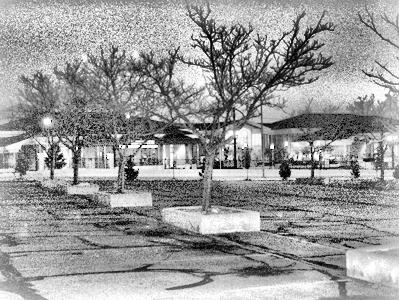
\includegraphics[width=\linewidth]{9/images/LC1_71.png}
          \caption*{Local histogram equalisation with $71\times 71$ bin}
          \label{fig:totalpowervst}
        \end{minipage}
        \begin{minipage}{.45\textwidth}
          \centering
          \includegraphics[width=\linewidth]{9/images/LC1_global_71.png}
          \caption*{Global histogram equalisation}
          \label{fig:totalpower2}
        \end{minipage}
        %\caption{}
        \label{fig:totalPower}
    \end{figure}
    $71\times 71$ gets closer to the global image compared to the small bin size images. Right middle block of global image also has low contrast near some hotel at the back, which is more clear in local image.
    \newpage
%--------------------------------------------------------------------------
%---------------------------------------------------------------------
  
    LC2:\\[10pt]
    \begin{figure}[H]
        \centering
        \begin{minipage}{.45\textwidth}
          \centering
          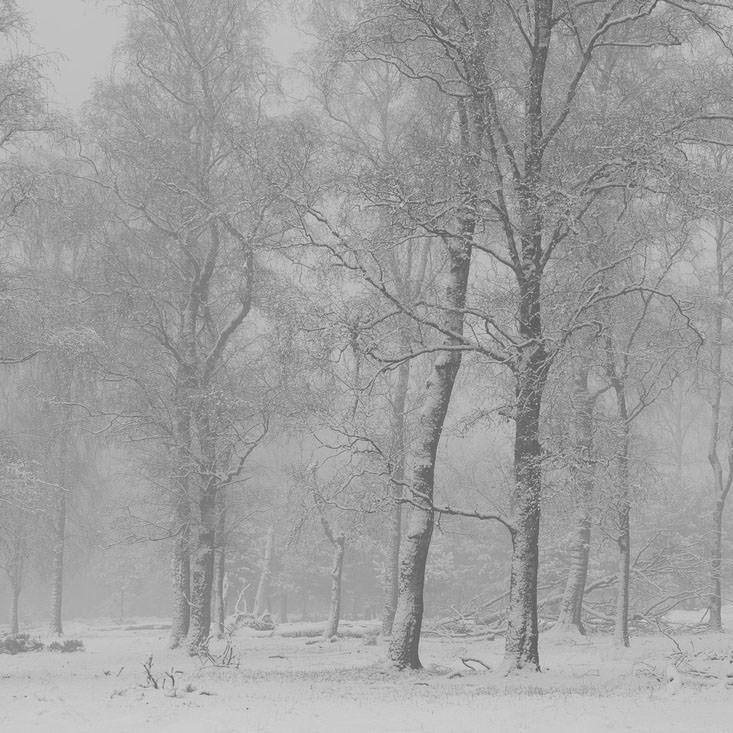
\includegraphics[width=\linewidth]{9/images/LC2.jpg}
          \caption*{Original LC2 image}
        \end{minipage}
    \end{figure}
    %-------------------------------------------------------
        
    \begin{figure}[H]
        \centering
        \begin{minipage}{.45\textwidth}
          \centering
          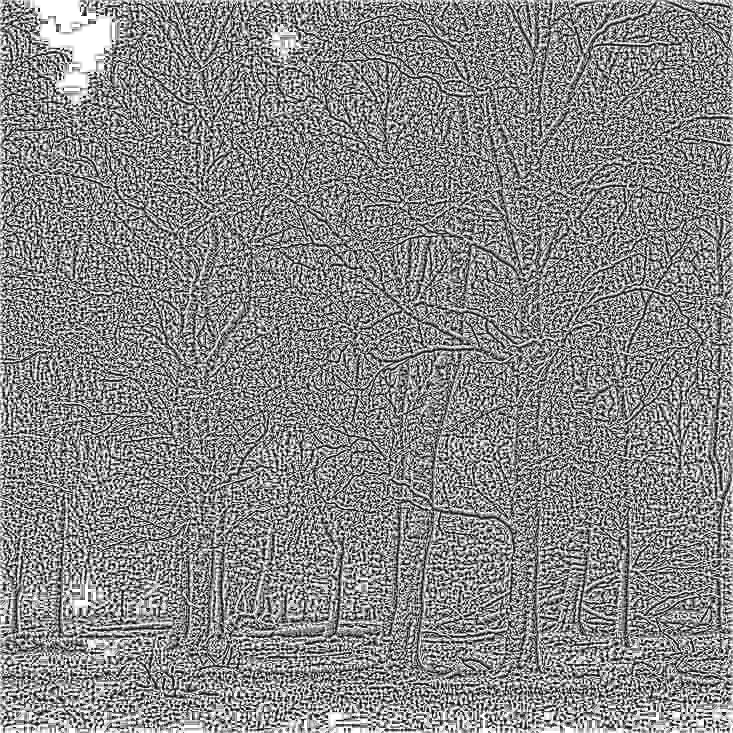
\includegraphics[width=\linewidth]{9/images/LC2_7.png}
          \caption*{Local histogram equalisation with $7\times 7$ bin}
          \label{fig:totalpowervst}
        \end{minipage}
        \begin{minipage}{.45\textwidth}
          \centering
          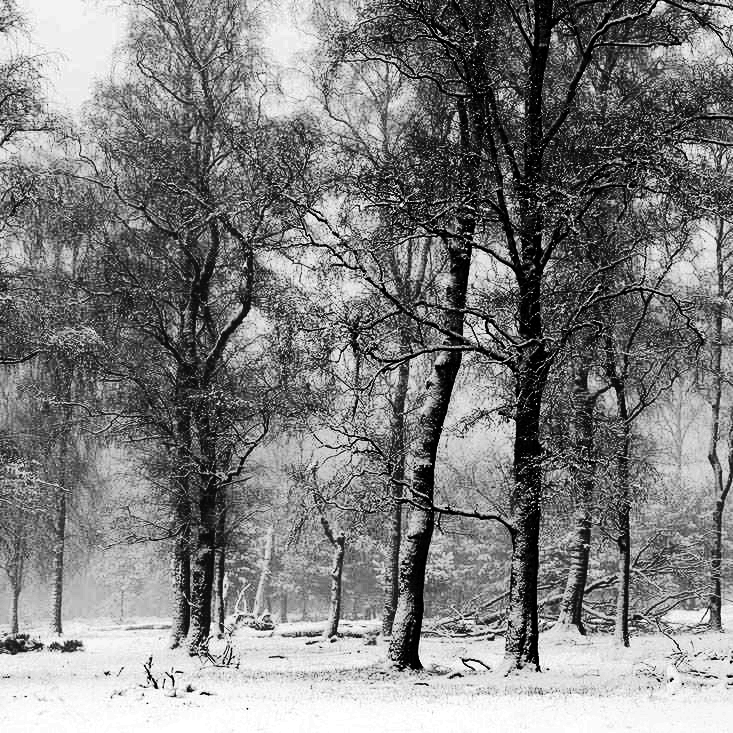
\includegraphics[width=\linewidth]{9/images/LC2_global.png}
          \caption*{Global histogram equalisation}
          \label{fig:totalpower2}
        \end{minipage}
        %\caption{}
        \label{fig:totalPower}
    \end{figure}
    Like in LC1 image $7\times 7$ locally equalised image isn't visually an improvement of the original image, but we do have some edge enhancements which may be used in an intermediate step of some other algorithm.
    
    %-----------------------------------------------------------------
    
    \begin{figure}[H]
        \centering
        \begin{minipage}{.45\textwidth}
          \centering
          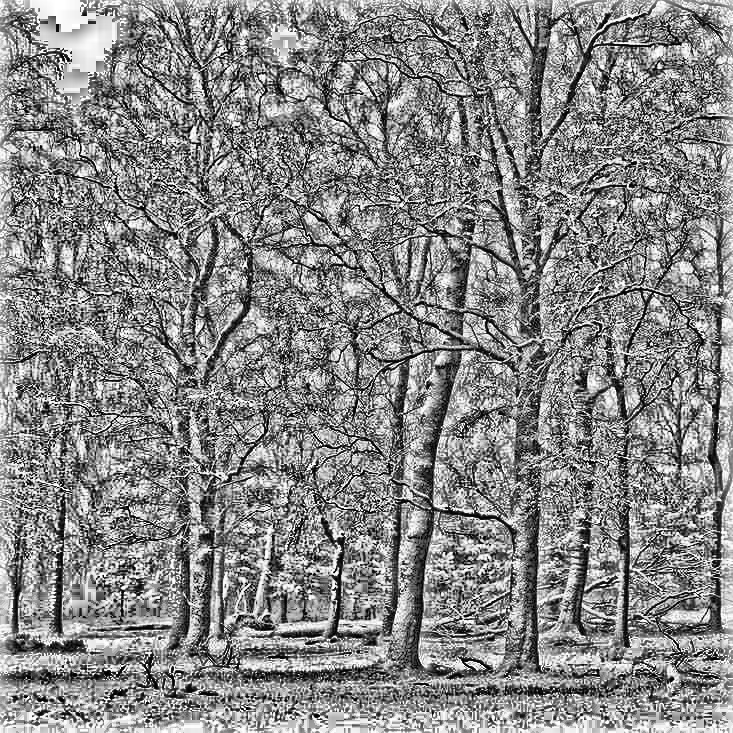
\includegraphics[width=\linewidth]{9/images/LC2_31.png}
          \caption*{Local histogram equalisation with $31\times 31$ bin}
          \label{fig:totalpowervst}
        \end{minipage}
        \begin{minipage}{.45\textwidth}
          \centering
          \includegraphics[width=\linewidth]{9/images/LC2_global_31.png}
          \caption*{Global histogram equalisation}
          \label{fig:totalpower2}
        \end{minipage}
        %\caption{}
        \label{fig:totalPower}
    \end{figure}
    Bottom part of the global image near the base of the tree is of low contrast with high intensity values(white), which has better contrast in the local image.
    %--------------------------------------------------------------------
    
    \begin{figure}[H]
        \centering
        \begin{minipage}{.45\textwidth}
          \centering
          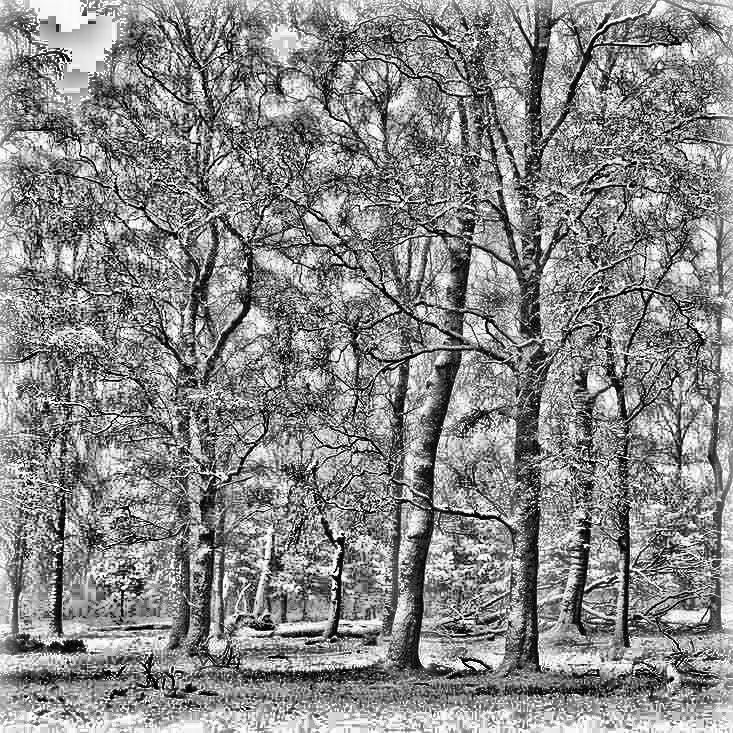
\includegraphics[width=\linewidth]{9/images/LC2_51.png}
          \caption*{Local histogram equalisation with $51\times 51$ bin}
          \label{fig:totalpowervst}
        \end{minipage}
        \begin{minipage}{.45\textwidth}
          \centering
          \includegraphics[width=\linewidth]{9/images/LC2_global_51.png}
          \caption*{Global histogram equalisation}
          \label{fig:totalpower2}
        \end{minipage}
        %\caption{}
        \label{fig:totalPower}
    \end{figure}
    In the block near the right edge is also of low contrast with low intensity values(black), the branches of the nearby trees can be estimated more accurately in the local image. 
    %------------------------------------------------------------
    
    \begin{figure}[H]
        \centering
        \begin{minipage}{.45\textwidth}
          \centering
          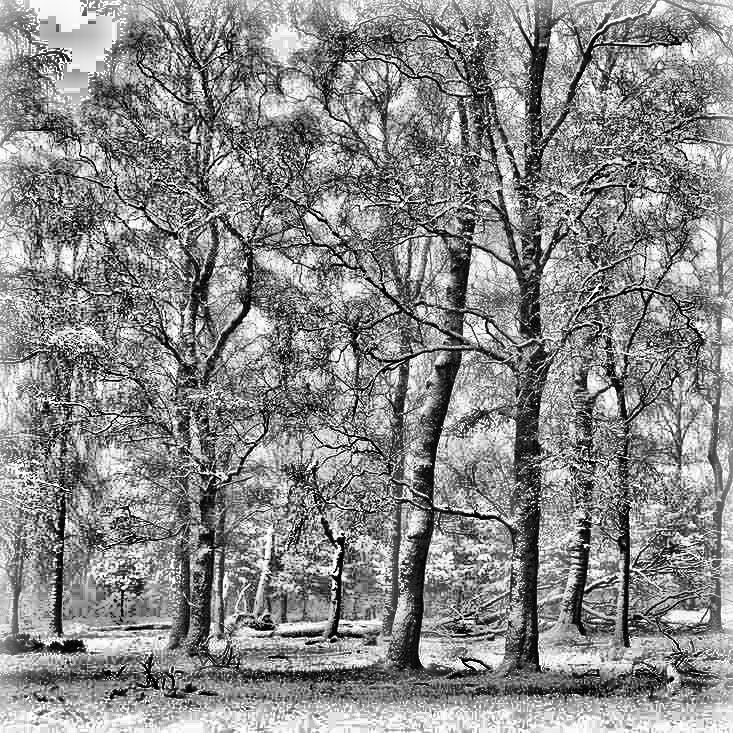
\includegraphics[width=\linewidth]{9/images/LC2_71.png}
          \caption*{Local histogram equalisation with $71\times 71$ bin}
          \label{fig:totalpowervst}
        \end{minipage}
        \begin{minipage}{.45\textwidth}
          \centering
          \includegraphics[width=\linewidth]{9/images/LC2_global_71.png}
          \caption*{Global histogram equalisation}
          \label{fig:totalpower2}
        \end{minipage}
        %\caption{}
        \label{fig:totalPower}
    \end{figure}
    In the left bottom block shown, we could identify a tree far away in the local image which may not be obvious in the global image because of low contrast of high intensity values.\\[20pt]
    %---------------------------------------------------------------
    For the given LC1 and LC2 images, none of the local histogram equalised images have a better overall image enhancement than global histogram equalised images, but locally equalised images give some additional information if we narrow our focus to certain small regions. 
\end{itemize}

\end{document}